\chapter{The Project Context}\label{project_scope_transformations}
Up until this point COOP is already conceptually able to process simple test software consisting of a single source file (e.g. c/cpp) and whatever files it may include. When using the LibTooling suite we will actually create a \textit{Tool} instance, that comprises elements of the Clang compiler front-end. To obtain the ASTs we depend on through out our entire process we feed the source files to that Tool instance. It includes a preprocessor that will resolve an preprocessor directives. This means, that any include files will be correctly treated as parts of the compilation unit. This way we can think of the resulting ASTs as representations of the to-be object files.\\
Tings get tricky however as soon as we actually start to try operating on multiple files. The \textit{Tool} instance is perfectly able to sequentially process different source files and will produce ASTs for each of them. So while we are not necessarily facing any exceptions we will at this point at least run into strange and faulty behavior. We want and need to operate on project scope. Our entire optimization strategy depends on knowing what records and fields there are, as well as every single usage of them throughout our source files respectively.\\
The LibTooling suite is intended to perform modular source-to-source transformations, for example automated style checks/improvements. This works because while those tools can be given multiple source files, ther transformation criteria will never depend on shared state between the created ASTs. In terms of optimizations we effectively want to perform a link time optimization, so we can operate on the entirety of our target project's code.\\\\
Creating an AST for each translation unit will hurt us in terms of multiply defined AST nodes. For example when our project defines a \textit{Foo.hpp} file, that contains the class definition of class \textit{Foo} and we have two source files \textit{Foo.cpp} and \textit{main.cpp} both including \textit{Foo.hpp} we will already have multiple AST nodes for our Foo's class definition in our context, as well as all the AST nodes representing method and field declarations. We wouldn't care if our transformation criteria was modular, however searching the ASTs for record definitions will now yield two class definitions and without further clarification our routine will treat them separately as they are distinct AST nodes. This applies to virtually every type of AST node.\\
Also e.g. functions and methods might associate AST nodes that will be declared in their AST context, however their respective definitions could (and will often times) exist in an entirely other translation unit.\\\\
Source transformations are also affected, since Clang's \textit{Rewriter} utility class will not be able to behave correctly when operating on distinct AST nodes pointing to the same physical file (The Rewriter is the source transformation tool, provided by Clang). It wont necessarily break but if changes coming from different Rewriter instances affect overlapping segments of the source file strange things will happen (or no changes might be committed at all). Not to mention applying the same (redundant) changes coming from seemingly different AST nodes to the same physical file segments. So first of all we will need a proper 'file to Rewriter instance' mapping, which can easily be done.\\\\
AST nodes are able to be dereferenced into their \textit{Source Locations} which are Clang's mechanism to associate an AST node to a specific physical location in a specific file. All of the relevant information concerning the AST are represented in it's respective \textit{AST Context} e.g. which source files it represents (\textit{SourceManager}) or what language options need to be considered (\textit{LangOptions}). So whenever we want to change a specific code segment, instead of creating a Rewriter instance on the spot, we will first check, whether or not there already exists a rewriter instance that was assigned to a specific AST Context.\\
Ongoing we will need more sophisticated mechanisms to prevent redundant processes as well as correctly associate AST nodes, that depend on each other, exceeding their definition's AST contexts. To do so we will in certain terms logically link several AST's resembling the work, that would otherwise be done by the linker using the symbol table.

\subsection{Global AST Node Representations}
As mentioned before when working with multiple source files we will most likely encounter multiply defined AST nodes which resemble the same source code for different translation units. For us these are redundant nodes and whenever we happen to use redundant AST nodes we will produce blurred or plainly wrong results. For example consider \reffig{project_context}. When creating the function/member matrix discussed in \refsec{auto_oop_to_dod} we could end up counting all member expressions of one source file \textit{Foo.cpp} and account them to the class definition we found in \textit{Foo.hpp} for the \textit{AST Context 1}. The member expressions we find in \textit{main.cpp} we might account to the class definition node we found in \textit{Foo.hpp} but this time we refer to the AST node coming from \textit{AST Context 0}.
\begin{figure}[!htbp]
	\centering
	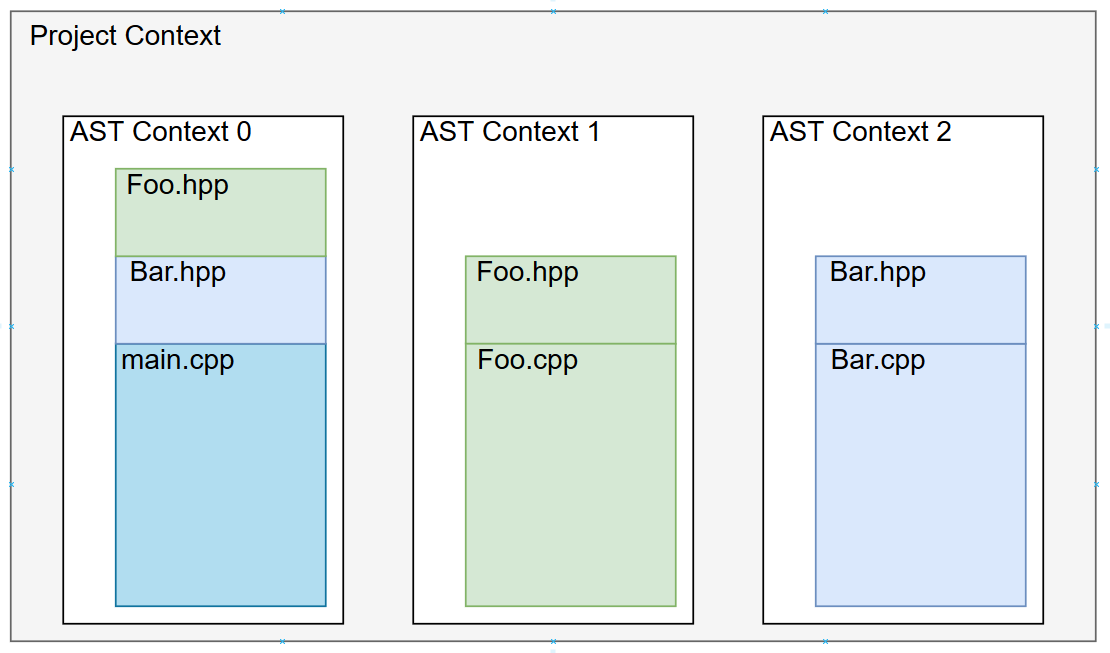
\includegraphics[width=0.6\textwidth, height=0.4\textwidth]{PICs/project_context}
	\caption{Visualization of how different AST contexts might include identical/redundant information when regarded in an abstract project scope.}
	\label{project_context}
\end{figure}
To ensure consistent association of possibly redundant AST nodes and logically unique entities, we need to somehow check whether or not AST nodes refer to the same source. Clang's AST node type \textit{clang::Decl} is the base for all declaration based AST nodes. It does provide functionality to retrieve a unique ID for a declaration, however that ID is only valid inside a single AST.\\
To distinguish different AST nodes and identify 'project scope duplicates' we need to somehow generate a unique ID for an AST node, that will reproduce the same result for each AST context. The entities name is not enough since logically different entities can share a name in different in different namespaces and even scopes. COOP will therefore use the nodes source locations. The one thing that each duplicate AST node will have in common is its reference to the physical source file, as well as its position inside that file. No other distinct Definition/Declaration, can share this trait. The appropriate information can be retrieved by consulting the AST context's source manager instance.\\
Even though an AST context will include the declarations that come with resolving preprocessor directives, the definitions of other source files won't be present in it. After all this is something the linker would do, in the following steps of actual compilation. So even though we can now identify duplicate declarations inside our project context, the 'link' of a declaration to its definition still has to be done manually by us.\\
This will actually happen in the \textit{Data Aggregation} step discussed in \refsec{data_aggregation} however only now we have the background to explain some interesting details. The matchers defined in \refsec{auto_oop_to_dod} will search for declarations or definitions depending on what we need of them. Whenever a matcher yields a possible candidate and invokes our callback routine, COOP will then create a wrapper object for virtually every node we want to remember.\\
These \textit{coop::ptr\_ID} wrappers contain a generic pointer to any kind of AST node, a unique identifier and a pointer to the relevant AST context. For each AST node type we need to remember, there will be a global container of \textit{ptr\_ID}s. The data aggregation's callback routines that are invoked when a matcher finds a relevant AST node, will now always generate an ID for the node they examine and register it in the global container, when no other ptr\_ID with the same unique ID is yet present.\\
From now on whenever an AST node is retrieved from the AST before doing anything else we will always first ask a \textit{coop::global<T>} container whether or not there is already an AST node, that represents this particular node. In most cases this already provides enough security for our demands, because most of the times we only ever care about counting entity occurrences. Theoretically it is possible now to globally register for example two distinct field declarations from the same record coming from different AST contexts, depending on the sequence in that they were found. And in most cases this will not even be a problem, as long as we are only interested in counting occurences and need to associate a e.g. member expression to a field declaration. However the ASTs are traversed and matched sequentially, so for example field and record declarations will be matched together and therefore point to a single AST context already as a result of their traversal sequence.\\
But whenever we need to depend on the AST nodes definition, because the definition contains valuable information, there is a problem. Functiondeclarations as well as record declarations might be forwarded/prototyped at one place but defined somewhere else (even in different files).\\\\
In this case we need to manually ensure, that we never process an AST node declaration, that can't find the appropriate definition. For example lets consider \reffig{project_context} again. Imagine \textit{Foo.hpp} declares a relevant function, that is then defined in \textit{Foo.cpp}. In case AST context 0 was created first, the moment we found the function declaration, we created the appropriate ID and remembered its AST context (AST context 0). After that, when traversing the AST 1 we would again find the function declaration, only this time we are able to associate it to a definition, because the AST context 1 encompasses the \textit{Foo.cpp} file. In this case we need to make sure that our global registry remembers the AST node from AST context 1. So we 'bend' the existing \textit{coop::ptr\_ID} node pointer and AST context pointer accordingly. Same goes for record definitions, as they are subject to forwarding. \refcode{bending} partly shows the callback routine, that is invoked by the AST matchers when they find an AST node of type \textit{clang::FunctionDecl} (a fucntion declaration).
\begin{lstlisting}[language=C++, name={Shortened excerpt of the callback routine, that registers function declarations for COOP in the data aggregation step.},label={bending}]
void coop::PrototypeBending::run(const MatchFinder::MatchResult &result){
	const FunctionDecl *proto = ...;
	const FunctionDecl *func = proto->getDefinition();
	
	if(!func){return;}

	std::string id = coop::naming::get_decl_id<FunctionDecl>(proto);
	
	auto global_f = coop::global<FunctionDecl>::get_global(id);
	if(global_f){
		global_f->ptr = func;
		global_f->ast_context = result.Context;
	}else{
		coop::global<FunctionDecl>::set_global(func, id, result.Context);
	}
}
\end{lstlisting}
In line 3 we determine whether this declaration is able to associate its definition. Next in line 7 we generate a unique ID for the record declaration, that we will use to determine whether or not there is already a node, that associates this declaration. If so this will be a declaration node coming from another AST, that will therefore not be able to associate this definition. In line 9 we ask the global registry whether it can return us a node that is registered with the id we made. If so we now have to bend the existing nodes pointer to the AST node that provides fill information and also associate the right AST context to the registry for that node. We can't just delete the existing ptr\_ID and create the correct one, as we must assume that at this point pointers to this ptr\_ID might have been created.

\subsection{Project contextual AST abbreviation}
\begin{wrapfigure}[17]{r}{.6\textwidth}
	\centering
	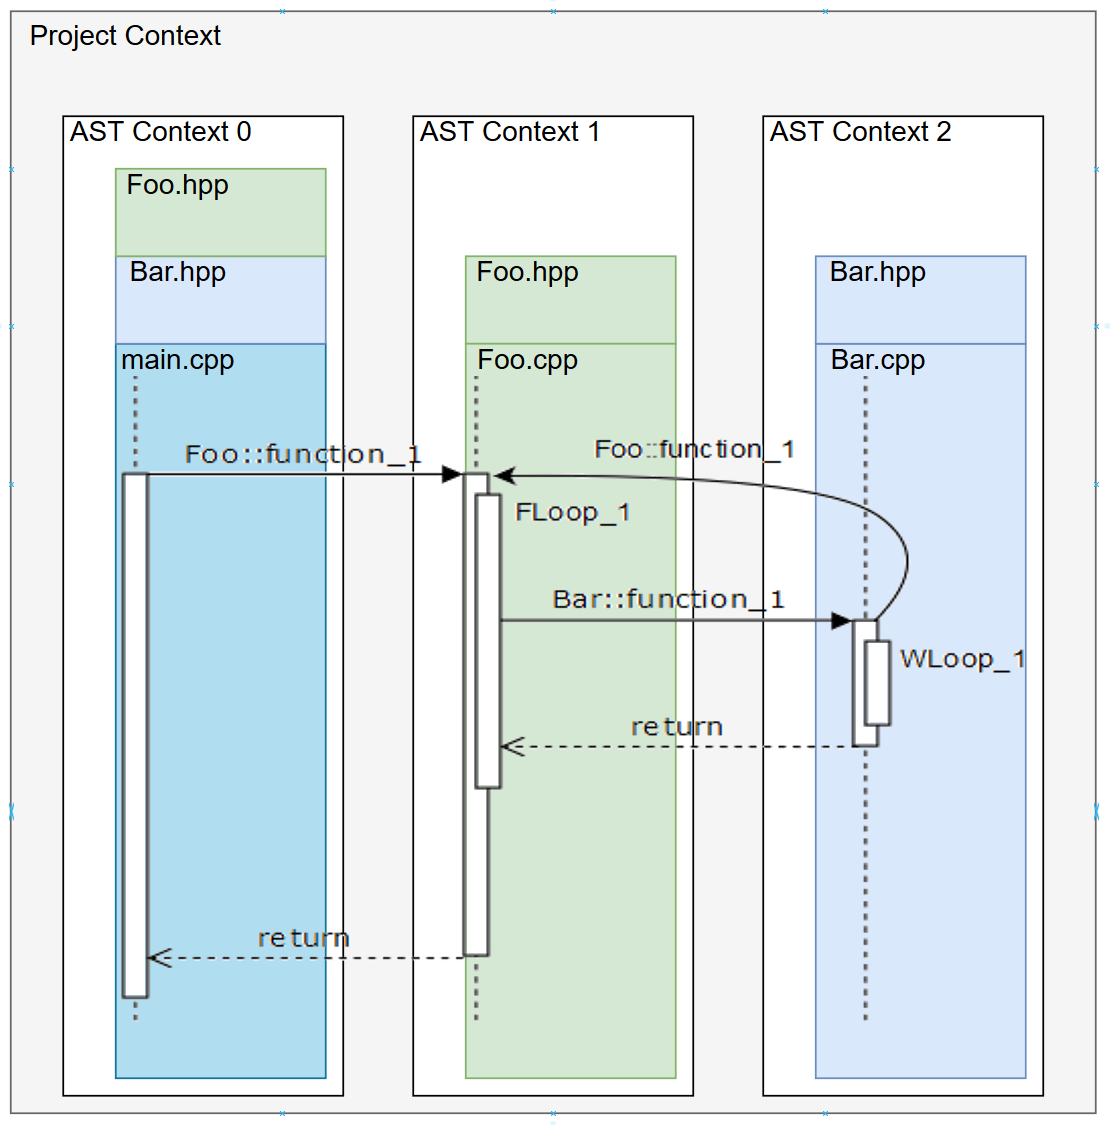
\includegraphics[width=.6\textwidth, height=0.42\textwidth]{PICs/recursion_context}
	\caption{Function calls and loops can interact in all sorts of forms in a program and recursion must be considered as it implicates similar behavior on access patterns as loops do.}\label{recursion}
\end{wrapfigure}
All of the above methods ensured, that our processes can interact on the global scale of the target project. The inherent problem we had, was that our optimization requires project contextual information, like what fields are used when and where and how often. We need to be able to link certain AST nodes from one AST to other nodes of other AST contexts. Now we can and its exactly what COOP needs to do next.\\
In order to create the function/loop member matrices we need to correctly depict the loop-depth of a field usage. Meaning how many scopes encompass this particular member expression that belong to a loop. This problem is not exactly trivial, since loops might be nested, functions might contain loops, loops might call functions that contain other loops \reffigp{recursion}. Theoretically this nesting of functions and loops is endless, it also might express recursion.\\\\
COOP's solution to this is to create a directed graph managing several AST nodes of functions and loops, that point to each other (given they assosiate each other in the original code). This graph would resemble the ASTs we created from the target project's translation units so why do it? Because in our own abbreviation of those ASTs we can 'merge' the different ASTs . Thanks to global registration of AST nodes we can now associate definitions to other definitions where we could only declare conceptual relation before. This resembles the steps the linker would normally do using a symbol table, although in this particular case we only do it for function calls and loops.\\
A node class \textit{fl\_node} (function/loop node) is used to hold either an AST \textit{clang::FunctionDecl} node or a \textit{clang::Statement} node if its a do/while or for loop. It also holds a list of child nodes, a count variable, that will later hold this particular nodes loop depth and indicators to whether it is involved in recursion.\\\\
After establishing the relevant links between the ASTs embodied in our AST abbreviation graph first of all we want to detect recursion. We search for recursion by traversing the graph and remembering the already visited nodes. When we follow a branch and end up on a node, we already have visited then we know it is the start of a recursive call. It is marked as such. Without further, more ambitious static analysis, there is no telling to what extend this recursive call resembles for example linear-, logarithmic- or even polynomial growth, so at this point any evaluation of its impact on the program is highly speculative. In \refsec{future_work} we will see that in order to make COOP viable much more static analysis would be needed.\\
In order to finalize the prototype we will merely treat recursive calls as another linear loop, so their 'depth' is equally important to a field's weight. With an evaluation of our programs data flow like this, that not necessarily resembles reality, but will hopefully mirror the proportions, we are now able to reason about a field's weight in terms of asymptotic notation \refsecp{metrics}.\\\\
However to correctly evaluate a field's relation to other fields of the same record, we still need to check whether fields are contextually related. In order to do this, we can again use our project context AST abbreviation. Whenever a function \textit{A} accesses a record \textit{Foo}'s fields \textit{m\_a} and \textit{m\_b} we already can establish, that \textit{m\_a} and \textit{m\_b} have contextual relation. But for each function/method \textit{B\_i}, that is called by \textit{A} we can't immediately decide whether it contains yet other fields of record \textit{Foo}, that should be regarded as contextually linked.\\
To establish correct field relations, we will traverse our AST abbreviation from bottom up. In this context this means, we start at functions that invoke no other functions. For each node we make sure that it's field usages are accounted to it's parent function calls. Assuming function \textit{A} uses \textit{Foo::m\_a} and it calls another function \textit{B} that itself uses \textit{Foo::m\_b} we will now treat \textit{A} as if it associates \textit{Foo::\_a} and \textit{Foo::m\_b}. This way when applying measurements, we derive from cohesion metrics \refsecp{metrics} we can correctly infer field relations. Remember, that cohesion metrics like \textit{LCOM4} only regard a record's methods. We operate project context wide, and therefore can't rely solely on comparing methods.\\
This is not due to cohesion metrics being sloppy, they are originally just used to make a statement on the records composition. We determine our own derivation of a cohesion metric, that reasons about a field's weight. For that we need not it's records cohesion index, but the fields' individual evaluation.\\\\
This sets the basis for our function/member matrices as we discussed in \refsec{data_aggregation}. As of now COOP is able to operate on a project that depends on linking several object files together and creating function/member and loop/member matrices, that encapsulate information for a record's fields to determine domain relations and usage frequency.


